

	\newpage
	\subsection{Lineare Interpolation} \label{chap:linearInterpolation}
	
	\sbreak
	\defi{
		\n 
		Die lineare Interpolation ist denkbar einfach. Wir sollen ja eine Funktion finden, die durch alle Stützpunkte hindurchgeht. Also können wir doch benachbarte Stützpunkte einfach mit Geraden verbinden und fertig.
		\n 
		Das Ergebnis ist eine Sammlung an Teilfunktionen, deren Funktionsintervalle genau an den Rändern jeweils anknüpfen.
	}

	\sbreak
	\methode{
		\n 
		Zwischen zwei benachbarten Stützpunkten $(x_i, y_i)$ und $(x_{i+1}, y_{i+1})$ definieren wir eine lineare Verbindung mit
		\begin{align}
			p_i(x) = (x - x_i) \cdot \frac{y_{i+1} - y_i}{x_{i+1} - x_i} + y_i \quad \quad x \in [x_i, x_{i+1}]
		\end{align}
		Machen wir das für alle $i = 0, \dots, n-1$, erhalten wir all solche Geraden, welche wir durch die Intervall Definitionen aneinander "kleben" können.
	}

	\sbreak
	\bsp{
		\n 
		Wir haben die Stützpunkte $(0, 1)$, $(1, 3)$ und $(3, 0)$. Wir möchten diese stückweise linear interpolieren.
		Wir definieren unsere zwei Teilfunktionen mit obiger Methode:
		\begin{align*}
			p_0(x) &= (x - x_0) \cdot \frac{y_{1} - y_0}{x_{1} - x_0} + y_0 &&	x \in [x_0, x_{1}] \\
				&= (x - 0) \cdot \frac{3 - 1}{1 - 0} + 1 &&	x \in [0, 1] \\
				&= x \cdot 2 + 1 &&	x \in [0, 1] \\
				& &&\\
			p_1(x) &= (x - x_1) \cdot \frac{y_{2} - y_1}{x_{2} - x_1} + y_1 &&	x \in [x_1, x_{2}] \\
				&= (x - 1) \cdot \frac{0 - 3}{3 - 1} + 3 &&	x \in [1, 3] \\
				&= (x - 1) \cdot -\frac{3}{2} + 3 &&	x \in [1, 3] \\
				&= -\frac{3}{2}x + \frac{9}{2}  &&	x \in [1, 3]
		\end{align*}
		\newpage
		\noindent Insgesamt könnten wir unsere Interpolationsfunktion (unser Ergebnis nennt man so) also folgendermaßen definieren:
		\begin{align*}
			g(x) = 
			\begin{Bmatrix}
				p_0(x); & x\in[0;1[ \\
				p_1(x); & x\in[1;3] \\
			\end{Bmatrix}
		\end{align*}
		Das bedeutet nichts anderes als, wenn man ein bestimmtes $x$ in $g(x)$ einsetzt, die Teilfunktion (also $p_0$ oder $p_1$) ausgesucht wird, in welchem Intervall sich das $x$ befindet. Wenn man beispielsweise jetzt $g(2)$ ausrechnen möchte, wird die zweite Teilfunktion ausgesucht, da $2 \in [1;3]$ gilt. 
		\begin{align*}
			g(2) = p_1(2) = -\frac{3}{2} \cdot 2 + \frac{9}{2}
		\end{align*}
		Klar könnte man in der Definition von $g(x)$ oben noch $p_0(x)$ sowie $p_1(x)$ einsetzen aber das spare ich mir mal \Laughey.
		\n
		Grafisch sähe das dann so aus:
		\begin{figure}[H]
			\centering
				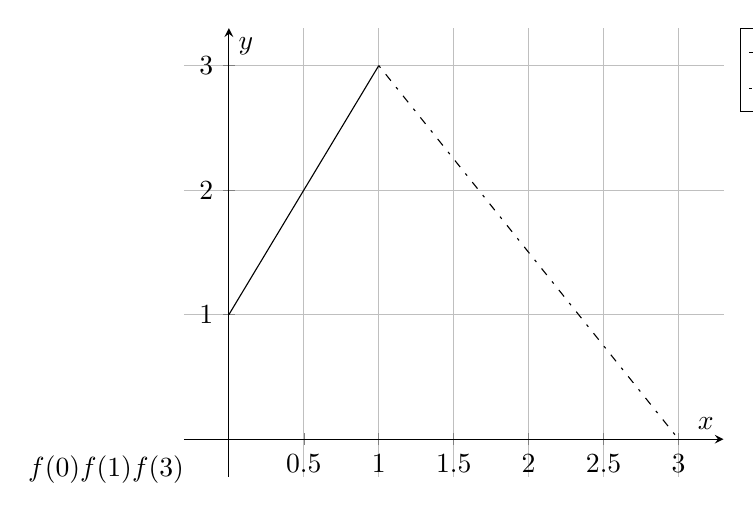
\begin{tikzpicture}
					\begin{axis}[
						axis lines=middle,
						xlabel=$x$,
						ylabel=$y$,
						enlargelimits,
						grid=major,
						cycle list name=color list,
						legend pos=outer north east,
						%ymin=-0.3,
						%xmax=5.8,
						%xticklabels={,,},
						%xtick={0, 1, 1.5, 2, 2.5},
						%yticklabels={,,},
						]
						\addplot[domain=0:1] {2*x + 1} node[left]{};
						\addplot[domain=1:3,dash pattern=on 1pt off 3pt on 3pt off 3pt] {-(3/2)*x + (9/2)} node[left]{};
						\tikzPointRight{$f(0)$}{0,1}
						\tikzPointRight{$f(1)$}{1,3}
						\tikzPointUp{$f(3)$}{3,0}
						\legend{$p_0(x)$, $p_1(x)$}
					\end{axis}
				\end{tikzpicture}
			\caption{Stückweise lineare Interpolation grafisch.}
		\end{figure}
	}

	\sbreak
	\wichtig{
		\n 
		Die erstellten Funktionen durch stückweise lineare Interpolation haben immer Knicke! Das bedeutet die Funktion ist nicht stetig differenzierbar!
	}
	